\documentclass[10pt,conference,compsocconf]{IEEEtran}

\usepackage{hyperref}
\usepackage{graphicx}	% For figure environment


\begin{document}
\title{Writing Scientific Papers and Software}

\author{
  Cheng Soon Ong\\
  \textit{Department of Computer Science, ETH Zurich, Switzerland}
}

\maketitle

\begin{abstract}
 The Higgs Boson challnege invovles using a large dataset to classify whether or not a particle is a Higgs Boson particle. We assessed various regression and classificaiton algorithms that could be used to predict the outcome and implemented some on the dataset. To further improve the results we preconditioned the data through various methods. Finally, a testing system was written to test all the combinations of preconditioning algorithms with the machine learning algorithms and output the one with least errors. 
\end{abstract}

\section{Introduction}
The Higgs Boson is a recently discovered very unpredictable particle. Through the particle collider at CERN, much data has been collected regarding the features of a decay processes when a Higgs Boson particle was present and was not present. We have analyze and automate several machine learning algorithms to predict whether or not the Higgs Boson particle is present given these features. 

When creating an algorithm there many choices for how to precondition the dataset and predict the output. We attempted to discover the optimal model by running various algorithms with various preconditioned datasets, and choosin the best one. We describe each of the techniques we use in the in the Precondition section and Classification section. 

\section{Preconditioning}
\label{sec:PreCond}

\subsection{Filling in Missing Data}
After observing the dataset we deduced that the values -999 and 0 were fillers for when the actual value is unknown. They occurred too frequently and were irregular compared to the other values of the same feature. We tried several approaches to filling in these gaps.
\begin{enumerate}
\item Mean/Median: We tried taking the mean of the rest of the data, ignoring the fillers, for every feature are replacing their mean or median. Either cases resulted in improvement in the accuracy.
\item Regression Filling
	We used the made the features datapoints and each datapoint a feature and used linear regression to fill the blanks. This method was more complex and time consuming to train but resulted in slightly better improvements in accuracy.
\item Delete features
	Eliminating the features with a 0 or -999 reduced the number of features to 19 which resulted in a poor accuracy.
\item Deleting samples
	181886 of the data points have a 0 or -999 so deleting all such points causes our algorithm to drastically underfit the model since the remaining sample size is too small, resulting in a poor accuracy.
\end{enumerate}

\subsection{Feature Extraction and Augmentation}
We tried a few computational methods of feature extraction with few results. These include removing features with a large variance or correlation. Intuitively, if a feature has a large variance it may seem that it is just background noise and can be ignored; however many natural measuerments have noise and outliers so it is not enough of a reason to discard the value. Furthermore, we tried visualizing the data and removing features that are highly correlated with each other. If one feature can predict another it seems unlikely that we need both features since they would be near linear combinations of each other and that is already accounted for with the weights. Finally, we wrote python scripts try removing one feature at a time and running the regression. This method seemed to have the most success and improved the accuracy the most.

\subsection{Normalization}
The data as given has a wide domain and is hard to statistically analyze, so we used several normalization techniques on the data.
\begin{enumerate}
\item Guassian Normalizer
\item Decimal Scaling
\item Minmax Normalizer
\item Guassian Outlier removal
\end{enumerate}

\section{Calssification Models}
\label{sec:ClassModels}

We used linear models and ran various classification algorithms

\subsection{Stochastic Gradient Descent}
detail parameters and stuff

\subsection{Least Squares}

\subsection{Ridge Regression}
This was the given figure example
\begin{figure}[tbp]
  \centering
  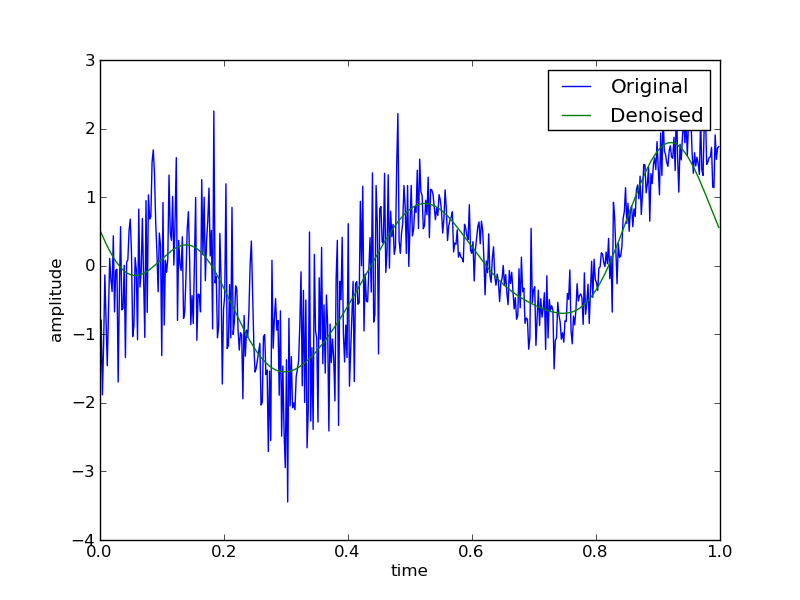
\includegraphics[width=\columnwidth]{denoised_signal_1d}
  \caption{Signal compression and denoising using the Fourier basis.}
  \vspace{-3mm}
  \label{fig:denoise-fourier}
\end{figure}
\begin{figure}[htbp]
  \centering
  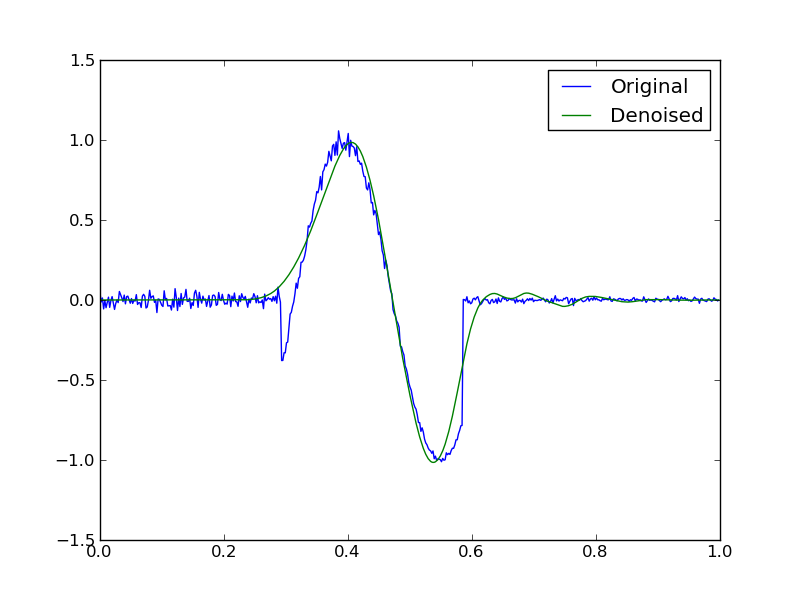
\includegraphics[width=\columnwidth]{local_wdenoised_1d}
  \vspace{-3mm}
  \caption{Signal compression and denoising using the Daubechies wavelet basis.}
  \label{fig:denoise-wavelet}
\end{figure}

Referring to Figure~\ref{fig:denoise-fourier} and
Figure~\ref{fig:denoise-wavelet}.

\subsection{Logistic Regression}
this is a citation ~\cite{anderson04,wavelab}.


\subsection{Testing and Results}
Describe how testing algorithms works
Use figures and maybe tables in results: See this example: Table~\ref{tab:fourier-wavelet}.

\begin{table*}[htbp]
  \centering
  \begin{tabular}[c]{|l||l|l|l|}
    \hline
    Basis&Support&Suitable signals&Unsuitable signals\\
    \hline
    Fourier&global&sine like&localized\\
    wavelet&local&localized&sine like\\
    \hline
  \end{tabular}
  \caption{Characteristics of Fourier and wavelet basis.}
  \label{tab:fourier-wavelet}
\end{table*}


\section{Tips for Good Software}
\label{sec:tips-software}

There is a lot of literature (for example~\cite{hunt99pragmatic} and
\cite{spolsky04software}) on how to write software. It is not the
intention of this section to replace software engineering
courses. However, in the interests of reproducible
research~\cite{schwab00}, there are a few guidelines to make your
reader happy:
\begin{itemize}
\item Have a \texttt{README} file that (at least) describes what your
  software does, and which commands to run to obtain results. Also
  mention anything special that needs to be set up, such as
  toolboxes\footnote{For those who are
  particularly interested, other common structures can be found at
  \url{http://en.wikipedia.org/wiki/README} and
  \url{http://www.gnu.org/software/womb/gnits/}.}.
\item A list of authors and contributors can be included in a file
  called \texttt{AUTHORS}, acknowledging any help that you may have
  obtained. For small projects, this information is often also
  included in the \texttt{README}.
\item Use meaningful filenames, and not \texttt{temp1.py},
  \texttt{temp2.py}. 
\item Document your code. Each file should at least have a short
  description about its reason for existence. Non obvious steps in the
  code should be commented. Functions arguments and return values should be described.
\item Describe how the results presented in your paper can be reproduced.
\end{itemize}


\subsection{\LaTeX{} Primer}
\label{sec:latex-primer}

\LaTeX{} is one of the most commonly used document preparation systems
for scientific journals and conferences. It is based on the idea
that authors be able to focus on the content of what they are
writing without being distracted by its visual presentation.
The source of this file can be used as a starting point for how to use
the different commands in \LaTeX{}. We are using an IEEE style for
this course.

\subsubsection{Installation}

There are various different packages available for processing \LaTeX{}
documents.
On OSX use Mac\TeX{}
(\url{http://www.tug.org/mactex/}). On Windows, use for example Mik\TeX{} (\url{http://miktex.org/}).

\subsubsection{Compiling \LaTeX{}}
Your directory should contain at least~4 files, in addition to image
files. Images should be in \texttt{.png}, \texttt{.jpg} or
\texttt{.pdf} format.
\begin{itemize}
\item IEEEtran.cls
\item IEEEtran.bst
\item groupXX-submission.tex
\item groupXX-literature.bib
\end{itemize}
Note that you should replace groupXX with your chosen group name.
Then, from the command line, type:
\begin{verbatim}
$ pdflatex groupXX-submission
$ bibtex groupXX-literature
$ pdflatex groupXX-submission
$ pdflatex groupXX-submission
\end{verbatim}
This should give you a PDF document \texttt{groupXX-submission.pdf}.

\subsubsection{Equations}

There are three types of equations available: inline equations, for
example $y=mx + c$, which appear in the text, unnumbered equations
$$y=mx + c,$$
which are presented on a line on its own, and numbered equations
\begin{equation}
  \label{eq:linear}
  y = mx + c
\end{equation}
which you can refer to at a later point (Equation~(\ref{eq:linear})).

\subsubsection{Tables and Figures}

Tables and figures are ``floating'' objects, which means that the text
can flow around it.
Note
that \texttt{figure*} and \texttt{table*} cause the corresponding
figure or table to span both columns.



\section{Summary}
Do this too.
The aim of a scientific paper is to convey the idea or discovery of
the researcher to the minds of the readers. The associated software
package provides the relevant details, which are often only briefly
explained in the paper, such that the research can be reproduced.
To write good papers, identify your key idea, make your contributions
explicit, and use examples and illustrations to describe the problems
and solutions.

\section*{Acknowledgements}
probs acknowledge class and stuff
The author thanks Christian Sigg for his careful reading and helpful
suggestions.

oh and see the code for how to do the bibliography

\bibliographystyle{IEEEtran}
\bibliography{literature}

\end{document}
